\documentclass[en]{../../../../../../eplexam}
\usepackage{../../../../../../eplunits}

\hypertitle{Synthesis of digital integrated circuits}{7}{ELEC}{2570}{2020}{Janvier}{All}
{Alice Borbáth \and Jean-Martin Vlaeminck}
{David Bol}

\setlist[enumerate]{label=(\alph*)}

\section{Business model}

\begin{enumerate}
	\item What is KPI-driven innovation?
	\item Give an example.
\end{enumerate}

\begin{solution}
Hint: look into the course, last slides.
\end{solution}


\section{Verification}

\begin{enumerate}
	\item What is assertion-based verification (ABV)?
	\item Why is it needed?
	\item How does it work?
\end{enumerate}

\begin{solution}
Hint: look into the slides. Don't forget to talk about the fact that we may have feedback based on the internal state or behaviour of the SoC.
\end{solution}


\section{Embedded programming}

\begin{enumerate}
	\item What is interrupt-driven programming?
	\item How does it save power compared to polling-based programming?
\end{enumerate}
Explain with illustrations.

\nosolution


\section{Robust HDL}

\begin{enumerate}
	\item What is the typical structure of a Register-transfer-level (RTL) Verilog code with only REG2REG paths? As an example consider a simple datapath with one pipelined stage.
	\item Sketch the corresponding gate-level schematic.
\end{enumerate}

\begin{solution}
Hint: the example should use a simple datapath with one pipelined stage.
A structure like a counter has a pipeline stage that forms a loop, and is not a correct example.
\end{solution}


\section{Design clocking}

Fig.~\ref{fig:ff} shows the schematic of a C$^2$MOS flip-flop gate.
\begin{enumerate}
	\item Explain its operation and illustrate it with a timing diagram.
	\item Explain the setup time concept and the reason why it is not null.
\end{enumerate}
\begin{figure}[h!]
	\centering
	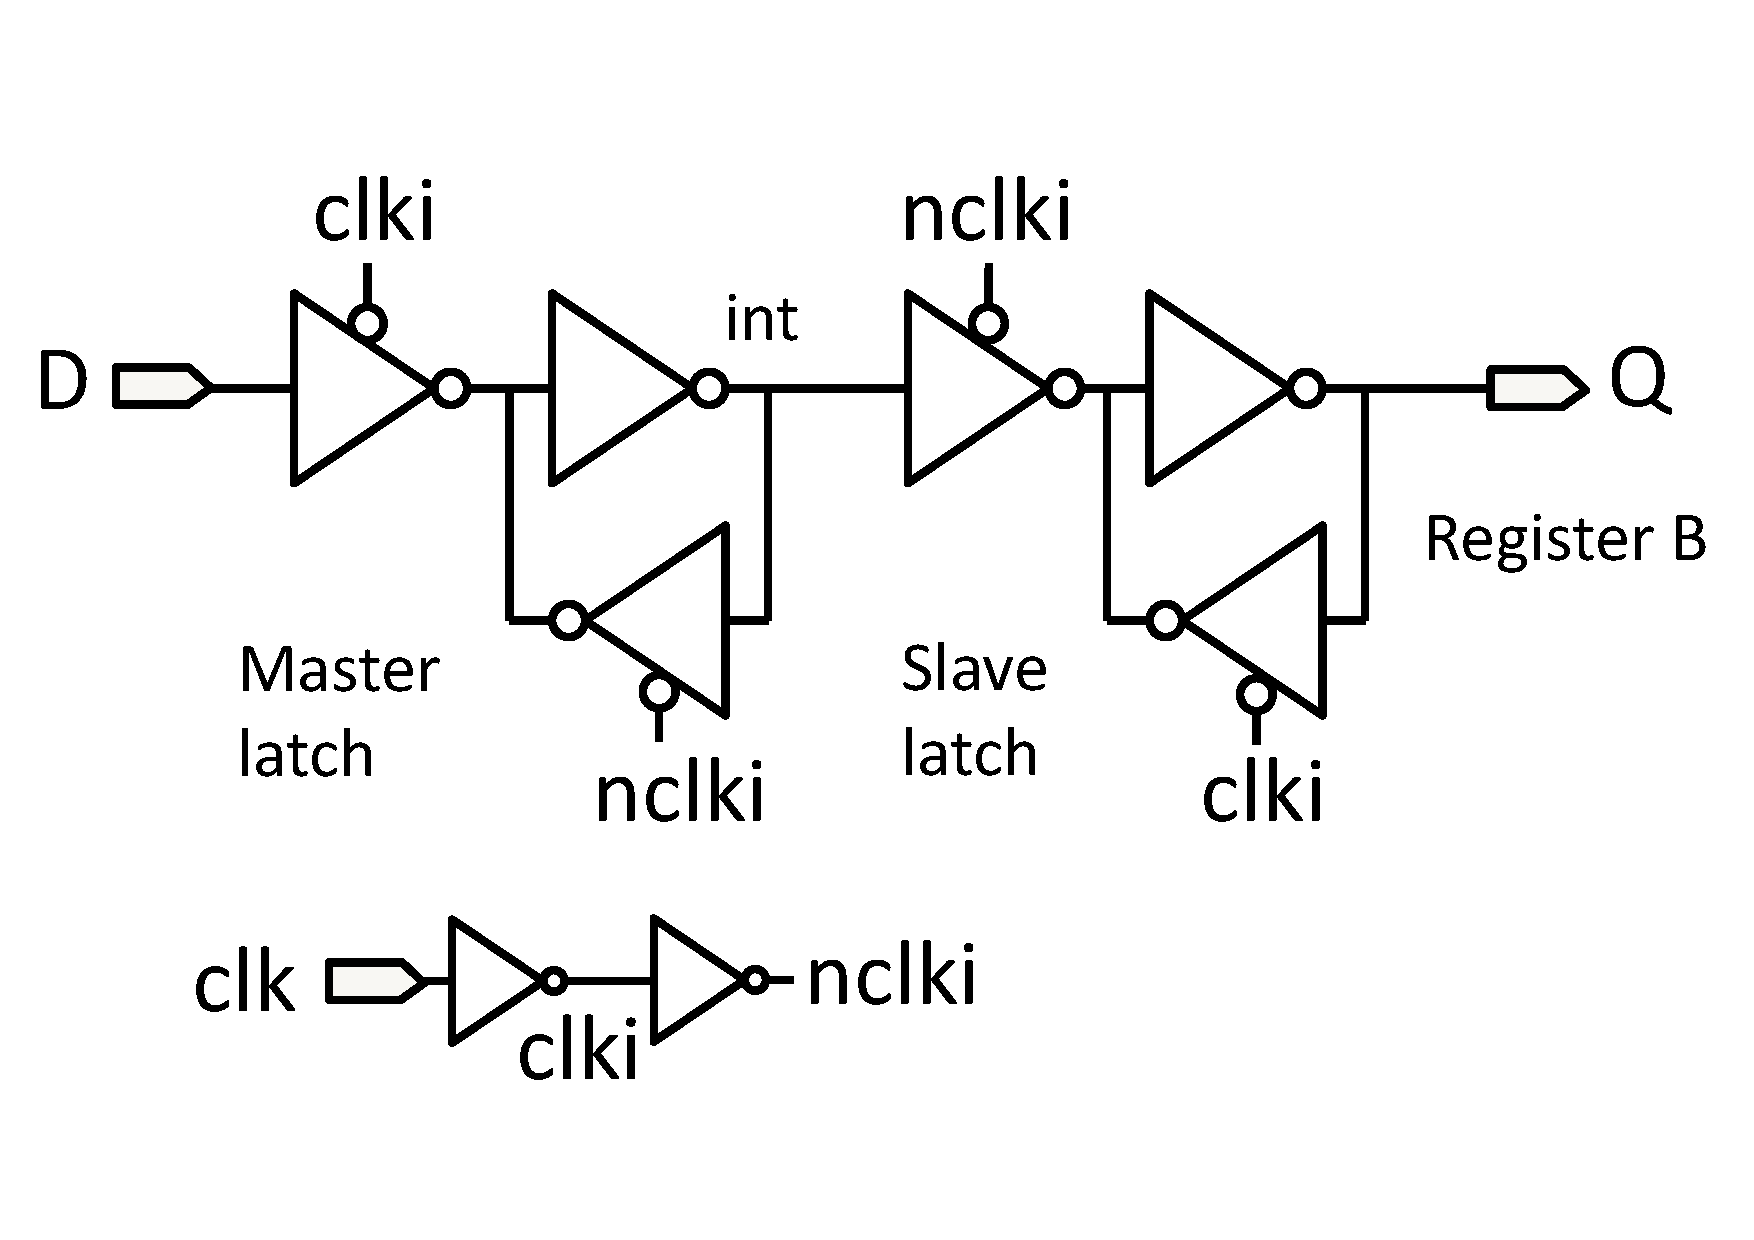
\includegraphics[width=0.8\textwidth]{img/flip-flop.pdf}
	\caption{}
	\label{fig:ff}
\end{figure}

\nosolution


\section{Memory architecture}

\begin{enumerate}
	\item What is the mux factor in an embedded memory hard macro?
	\item What is the read-access time (RAT) of an embedded memory hard macro?
	\item How is the RAT affected by the memory mux factor?
	\item Why?
\end{enumerate}

\nosolution


\section{Physical implementation}

\begin{enumerate}
	\item What does a clock tree in a digital IC?
	\item Which two performance metrics does it need to optimize?
	\item How is it implemented?
\end{enumerate}

\begin{solution}
Hint: need to talk about the role of the clock tree; the fact that we want to have a limited clock skew; the fact that we want a limited clock slew/transition (i.e., a sharp edge); and that we can put buffers to improve all of this.
\end{solution}


\section{Technology scaling}

\begin{enumerate}
	\item How does constant-field technology scaling increase subthreshold leakage power?
	\item Give a solution at the technology level.
	\item Give a solution at the circuit design level.
\end{enumerate}

\nosolution


\section{DSP}

How many cycles, PMEM and DMEM accesses do we need to compute one output sample of an N-tap FIR filter with a Von Neumann general-purpose processor (GPP)? Justify your answer with a pseudo assembly code.

\nosolution


\section{Pixracer project}

To avoid having to reprogram the SoC every time through JTAG,
we want to study the impact of replacing the imem SRAM by a Flash macro.
The base system uses a single block of 32kB SRAM for the imem,
and another one for the dmem, runs at \SI{50}{MHz}, has a power consumption of
around \SI{1.5}{mW}, \SI{0.65}{mW} for the imem and \SI{0.32}{mW} for the dmem.
In the technology used, we have access to only one Flash macro, of 32kB.
This macro has a RAT of \SI{5}{ns}, a write time of \SI{1}{ms},
and consumes \SI{1}{nJ} per write cycle, \SI{80}{pJ} per read cycle,
the idle energy is \SI{10}{pJ} per cycle, and has \SI{10}{uW} of leakage power.
In the question, the hierarchical power consumption report generated by Design Compiler is available.
\begin{enumerate}
	\item Determine the impact of replacing the imem SRAM by a Flash imem on the power.
	\item How can we reduce the power overhead of this Flash memory (give one method)?
\end{enumerate}

\nosolution


\end{document}
